.% -*- mode: latex; mode: linkd; mode: auto-fill; mode: flyspell;-*-
% Index
% (@> "Introduction")
% (@> "Collaboration")
%   (@> "Advantages of collaboration")
%    (@> "Knowledge sharing")
%    (@> "Richer forms of communication")
%    (@> "Share Resources")
%   (@> "Classification of CSCW Systems")

\chapter{Collaborative modelling}
\label{chap-four}

% (@file :file-name "thesis.tex")

% (@* "Introduction")
The objective of Coglaborate is to provide a collaborative modeling
environment for the cognitive science community. It does so by
mounting ACT-R on the Biobike infrastructure. The system currently
supports collaboration asynchronously. This means that a certain
researcher can develop a model and share it with his colleague, who
can work on that model separately and share it with other individuals.

% This chapter discusses the advantages provided by a shared environment
% such as Coglaborate. It also tries to provide a framework for the future
% development of Coglaborate, by providing the means that we used to come
% up with the requirements for this system.

This chapter starts off with a discussion about collaborative
systems. Which is then followed by a discussion about biobike, its
objectives and which part of the spectrum of the collaborative systems
it fits into. 

\section{Collaboration}
% (@* "Collaboration")
%explain why is collaboration required. 
Collaboration is the key to building large structures in almost all
human endeavors be it in the fields of either the arts or
sciences. Collaboration permits breaking down large unwieldy tasks
into more manageable chunks of work. It permits sharing of knowledge
and resources. Computer networks have provided us with a means of
communication between users of computers. This as a result has led to
an area of research that studies how computers can help users
communicate their ideas through computers and therefore use computers
as a means of collaboration, this field is commonly known as Computer
Supported Collaborative Work (CSCW).

\subsection{Advantages of collaboration using computers}
% (@* "Advantages of collaboration")
% Advantages of using computers in collaboration: Describe why you
% need this
We have three outcomes as a result of using computers to support
collaboration. They assist is sharing knowledge, for example consider
a Wiki. No other means that we currently know of would enable us to
share knowledge as freely and easily. They enhance communication
by allowing us to share richer content like video with each
other. Finally they allow us to share resources such as processing
power and storage capacity. Each of these outcomes have their
advantages that are discussed in detail below.

% (@* "Knowledge sharing")
The ability to share knowledge through computers helps us save
time. For example if a researcher develops a model of a certain
phenomenon on a computer and shares it with the community. Some other
person working on an extension of the project would save the time
taken to build this part of the model in the first place. And since we
are sharing knowledge, collaboration through computers lends it self
easily to be used as a pedagogical tool. For instance consider an
author of a textbook. He can easily create content, such as
presentations or write programs to demonstrate concepts, and can share
it off his website. This information can later be used by other
student and teachers to either learn more effectively and to improve
the way they teach respectively. Sharing knowledge also implies
sharing data. Running certain experiments can be time consuming and/or
costly. For example consider weather simulations a researcher in one
lab could simulate a scenario and make the data for the same available
for others doing so would help others working the area save time and
cost by not having to run that experiment again.

% (@* "Richer forms of communication")
Collaboration through means of computer provides us with richer forms
of communication that has not been available to us before. Apart from
allowing audio based communication, it provides us with means for
video based communication. As a result we can communicate with each
other more comprehensibly and that in turn avoids transfer of
ambiguous information. For example we have systems currently that help
us share screens, such systems could be used, for instance, by a
customer to clearly communicate his requirements to a vendor, who may
be in a different geographical area unambiguously. 

% (@* "Share Resources")
The ability to tie up computers together allows us to share
resources. This could either be in the form of hardware, where a power
server or servers are shared by many people or in the form of human
resources where people from different geographical locations can
collaborate effectively.

% 1) Easier to share knowledge:
%    a) Talk about sharing data,
%    b) code,
%    c) reuse of knowledge
% 2) Communication
%    a) Provides communication: wiki, 
% 3) Repository of knowledge
%    a) Store old knowledge
% 4) Hardware sharing
%    a) More powerful hardware at a common place
%    b) Cost change

\section{Classification of CSCW systems}
% (@* "Classification of CSCW Systems")

According to \cite{journals/iwc/Rodden91} there are two
characteristics of all CSCW systems namely, the form of interaction
and the geographical nature of the users. 

The form of interaction can be described as the method by which users
of a groups working together interact. This could either be
synchronously where every member of a group contributes in real time
an example of such a situation is brain storming. Another form of
interaction is asynchronous interaction. In such a form of interaction
the members of the group with one another with out the presence of
other members of the group. An example of this can be a group of
students collaborating with each other on a homework problem via a
message board.

The geographical nature of the users describes if the users interact
with each other remotely for example consider the case of developing
the linux kernel, developers and testers working on the kernel worked
with each other from geographically disparate locations. It could
also describe if the users are co-located, an example of this could be
users using a meeting room system like Colab\cite{Stefik:1987:BCU}. 

\begin{figure}[htp]
  \caption{Classification of CSCW systems\cite{journals/iwc/Rodden91}}
  \centering
  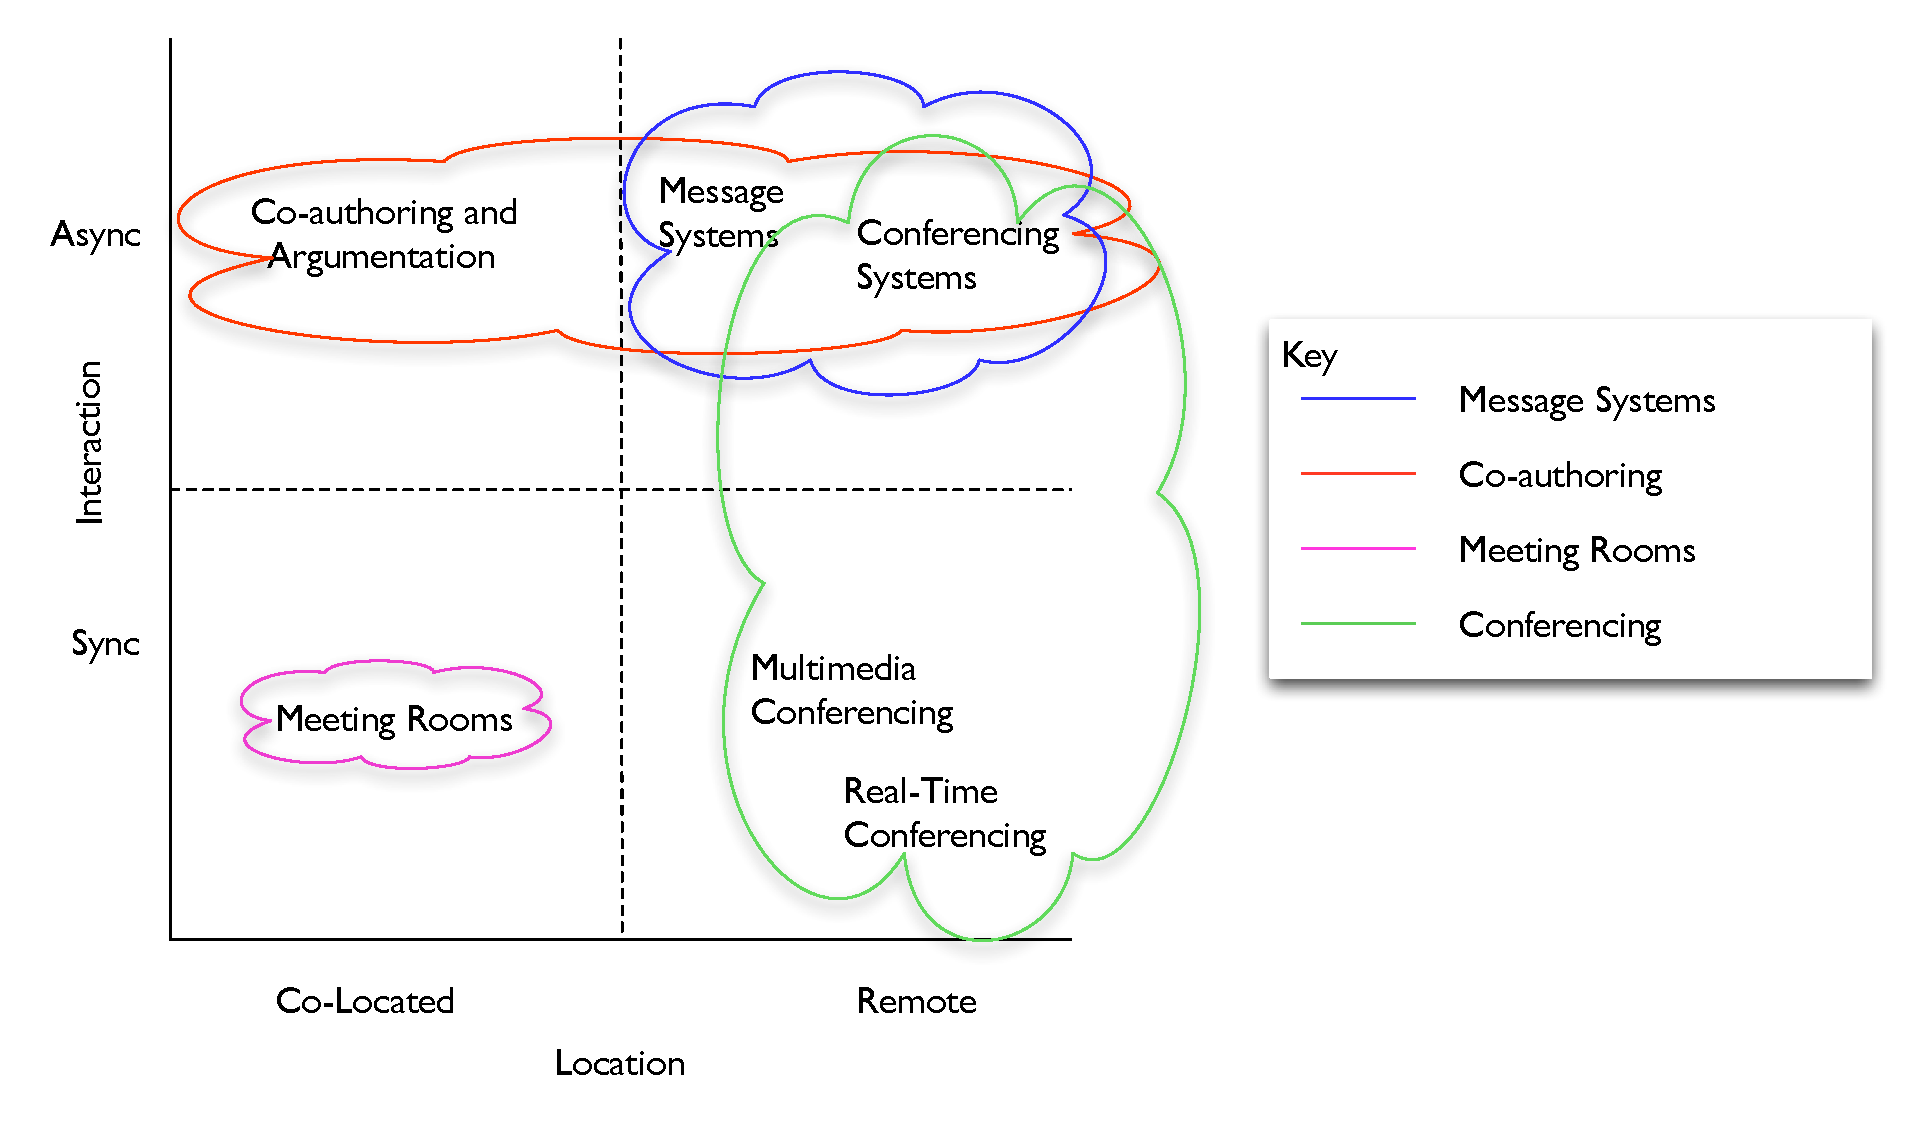
\includegraphics[width=140mm]{CSCWClass.eps}
  \label{CLASS_CSCW}
\end{figure}

\subsection{Message Systems}

Message systems derive their origins from e-mail based systems. The
factor that differentiates message systems from email based systems is
that message systems try to attach more semantic data to the messages
they process. Most of these systems use the object model to represent
messages. To instantiate messages the user fills in data context
specific data into slots, this data is used by the system to carry out
further processing by the system. Example of message systems include
COSMOS\cite{conf/cscw/BowersC88} and Information Lens\cite{Malo87a}. 

COSMOS represented research being carried out in the European CSCW
community. COSMOS was a project in the UK to design and develop a
configurable message system that supported structured group work. The
system was developed with a focus on specifying the users
communicative work in the form of participants actions. Group activity
tasks were represented in the system using the concept of
\emph{communication
  structures}(CS)\cite{conf/cscw/BowersC88}. Communication structures
were further described using a structure definition language(SDL). The
tasks that a COSMOS system was capable of carrying out was defined by
the communication structures defined in the system. The COSMOS system
also defines roles for users or agents, message objects, actions,
rules and actions in context of the work being carried out. Any
communication activity by the user is instantiated when the user
creates an instance of a communication structure. The user does this
by filling in the data required by the communication
structure. Further communication occurs by an exchange of messages
between users who compose a specific role mentioned in the
communication structure.

The Information lens on the other hand take a less formal
approach\cite{journals/iwc/Rodden91}. The aim of the author to develop
information systems that minimized information overload on the users
of the system that was caused by the amount of messages that were sent
to a user. The key ideas that defined Information lens were


\begin{itemize} 
  \item \emph{ Use of semi-structured messages to represent data:} The messages were represented as a set of semi-structured data
  called frames. A frame was a template that included information for
  date, time, place, organizer and any other unstructured data. This
  idea played an important role because; semi-structured messages make
  it easier for the computer to parse messages, according to informal
  studies conducted by the author of the paper\cite{Malo87a} people do
  most of their processing on a set of unstructured information and
  finally providing semi-structured fields enables authors to put in
  more context related information.

\item \emph{The use of production rules:} The system used sets of
  production rules each of which might contain multiple levels of
  reasoning that specify the reasoning of messages.

\item \emph{Use of specialized editors for creating and editing
    message templates and productions: } The authors of the system
  attempted to make the system more user friendly by providing
  multiple editors to create and edit message templates and
  productions.
\item \emph{Use of frame inheritance:} Using frame inheritance in
  messages allows messages to be specialized very easily
\item \emph{Introducing the system slowly to the users:} The authors
  believed that the introduction and evolution of a group work system
  can be useful if it is introduced slowly to users and encouraging
  users to switch to the system by rewarding users who switch to the
  system by providing additional benefits.
\end{itemize}

The message templates consisted of forms having fields where
information could be filled. The messages were edited using a display
oriented editor. The users constructed the IF part by specifying the
conditions that were required by a rule to satisfy condition by
combining specific conditions using logical operators like and, or and
not. The users used message handling primitives like move, delete,
save, etc. to specify the action to be taken on that message.

\subsection{Conferencing systems}
Conferencing systems found their advent in the 1970s when the US
government was looking for a way to deal with emergencies. EMISARI\cite{Hilt78a}
(Emergency Management Information System and Reference Index) was
the result of this effort. It consisted of two main ideas that even
today form the back bone of current conferencing systems, illustrated
in figure \ref{CONF_SYS}. This model
of communication allowed users to interact through a shared
information space, but at the same time it allowed user to interact
individually with one another. 

\begin{figure}[htp]
  \caption{Communication in a conference system\cite{journals/iwc/Rodden91}}
  \centering
  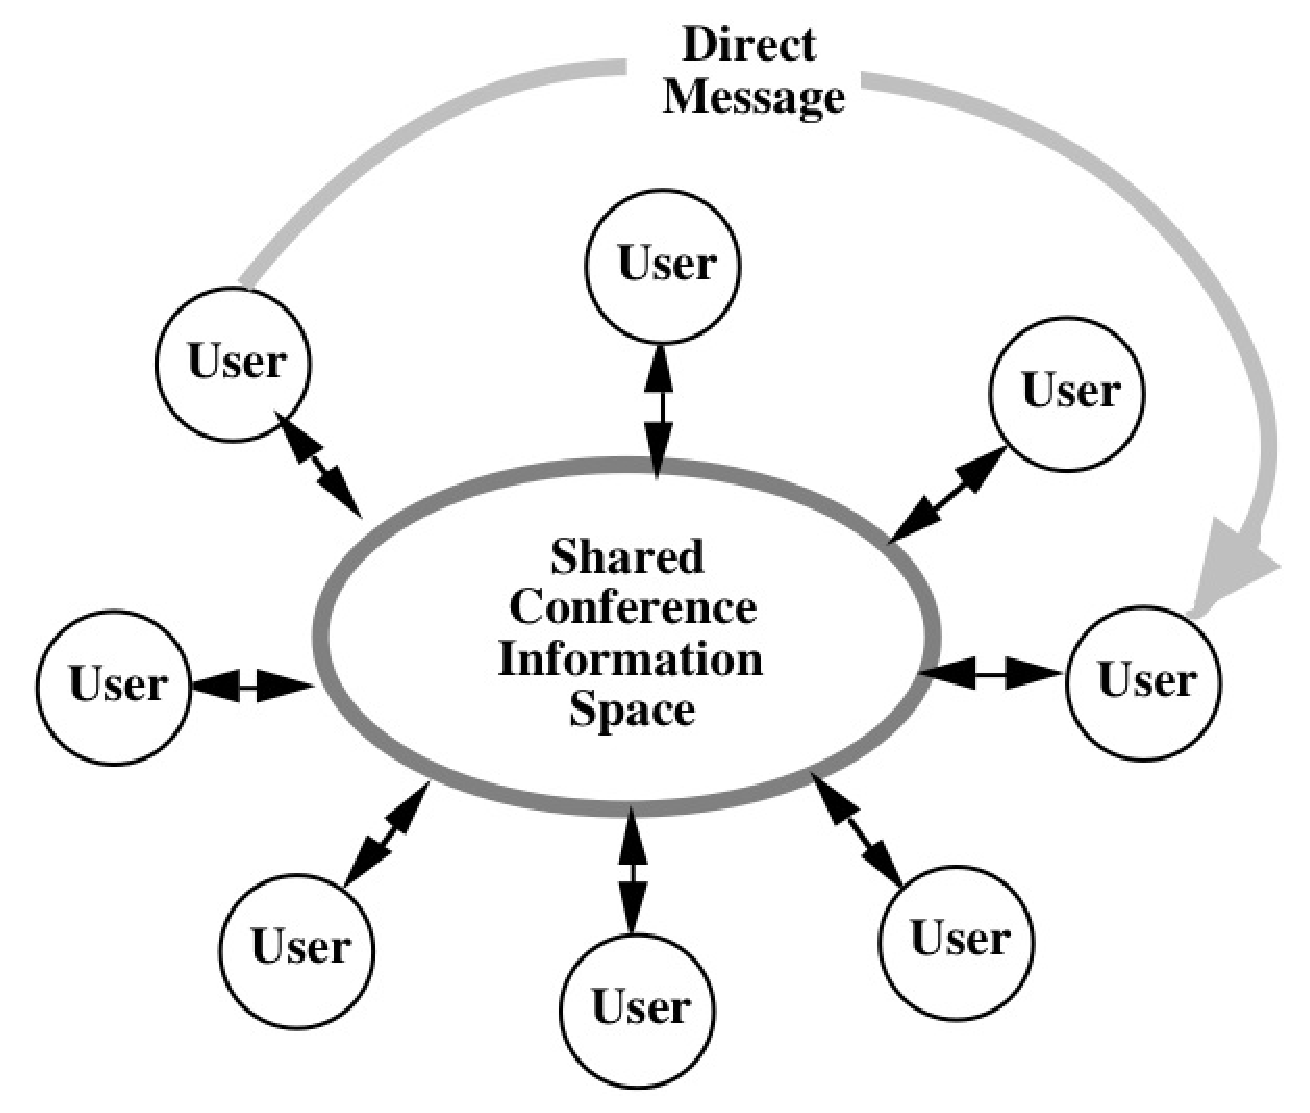
\includegraphics[scale=.5]{ConfSys.eps}
  \label{CONF_SYS}
\end{figure}

Roden cites the existences of two characteristics of the shared
information space for the existence of a number of forms of conference
systems. These characteristics are the type of information available to
be shared and the form of interaction. The users can use the system
asynchronously over a long period of time or synchronously in real
time. With the advent of newer formats of representing data the system
can use a wide range of media to represent information.

\subsubsection{Traditional conferencing systems}
Traditional conference systems were extensions of email systems . The
users of the system could subscribe to various conferences and the
system would send him or her messages as comments were posted. These
were different from mailing lists in that they allowed discussions to
be moderated by users and also provided flexibility in the way
conferences were created. Examples of traditional conference systems
include NOTEPAD by InfoMEDIA Corp,  Confer a conferencing system
developed at the university of Michigan.

\subsubsection{Real-time conferencing systems}

Real-time conferencing enables an instantaneous transfer of ideas and
flow of information between participants of the conference. Real-time
conferencing is important in situations that require real-time
participation by participants. RTCAL\cite{SG85} was a system developed
at the MIT Laboratory for Computer Science. It supported scheduling
meetings by building a shared workspace of information from the
participants calendars. Although it did not provide a tool that
automatically selected time for meetings, it provided a set of
decision support tools to help schedule meetings. RTCAL demonstrated a
number of features that are still relevant and applicable to most
real time conferencing systems today, most notable Microsoft Live
Meeting. 

Real-time conferencing systems may sometime also provide the user with
the facility to share screens. These are called shared screen
systems. Much of the work on shared screen systems are developed on
the work of Colab\cite{Stefik:1987:BCU}. Yuuguu can be cited as an
example of an instant screen sharing system.

\subsection{Meeting Rooms Systems}
% Describe meeting room systems. What they support.

% Another factor about meeting room systems

Meeting room systems find their roots back to a set of systems called
Group Decision support systems(GDSS). Kraemer\cite{KraKin88} cites
DeSanctis and Gallupe\cite{DG85} to define Group decision support
systems as ''an interactive computer-based system that facilitates the
solution of unstructured problems by a set of decision makers working
together as a group.'' The eventual aim of these systems was to help
groups improve their decision making process by providing a structured
process and a set of tools that would help groups come to beneficial
decisions.

The objective of meeting room support systems is to enable
collaboration between co-located groups of participants. It is
typically arranged in a meeting room having a large projector along
with a number of individual terminals, figure \ref{meeting_room_fig}
illustrates this arrangement. 

\begin{figure}[htp]
  \caption{Arrangement of a meeting room system\cite{journals/iwc/Rodden91}}
  \centering
  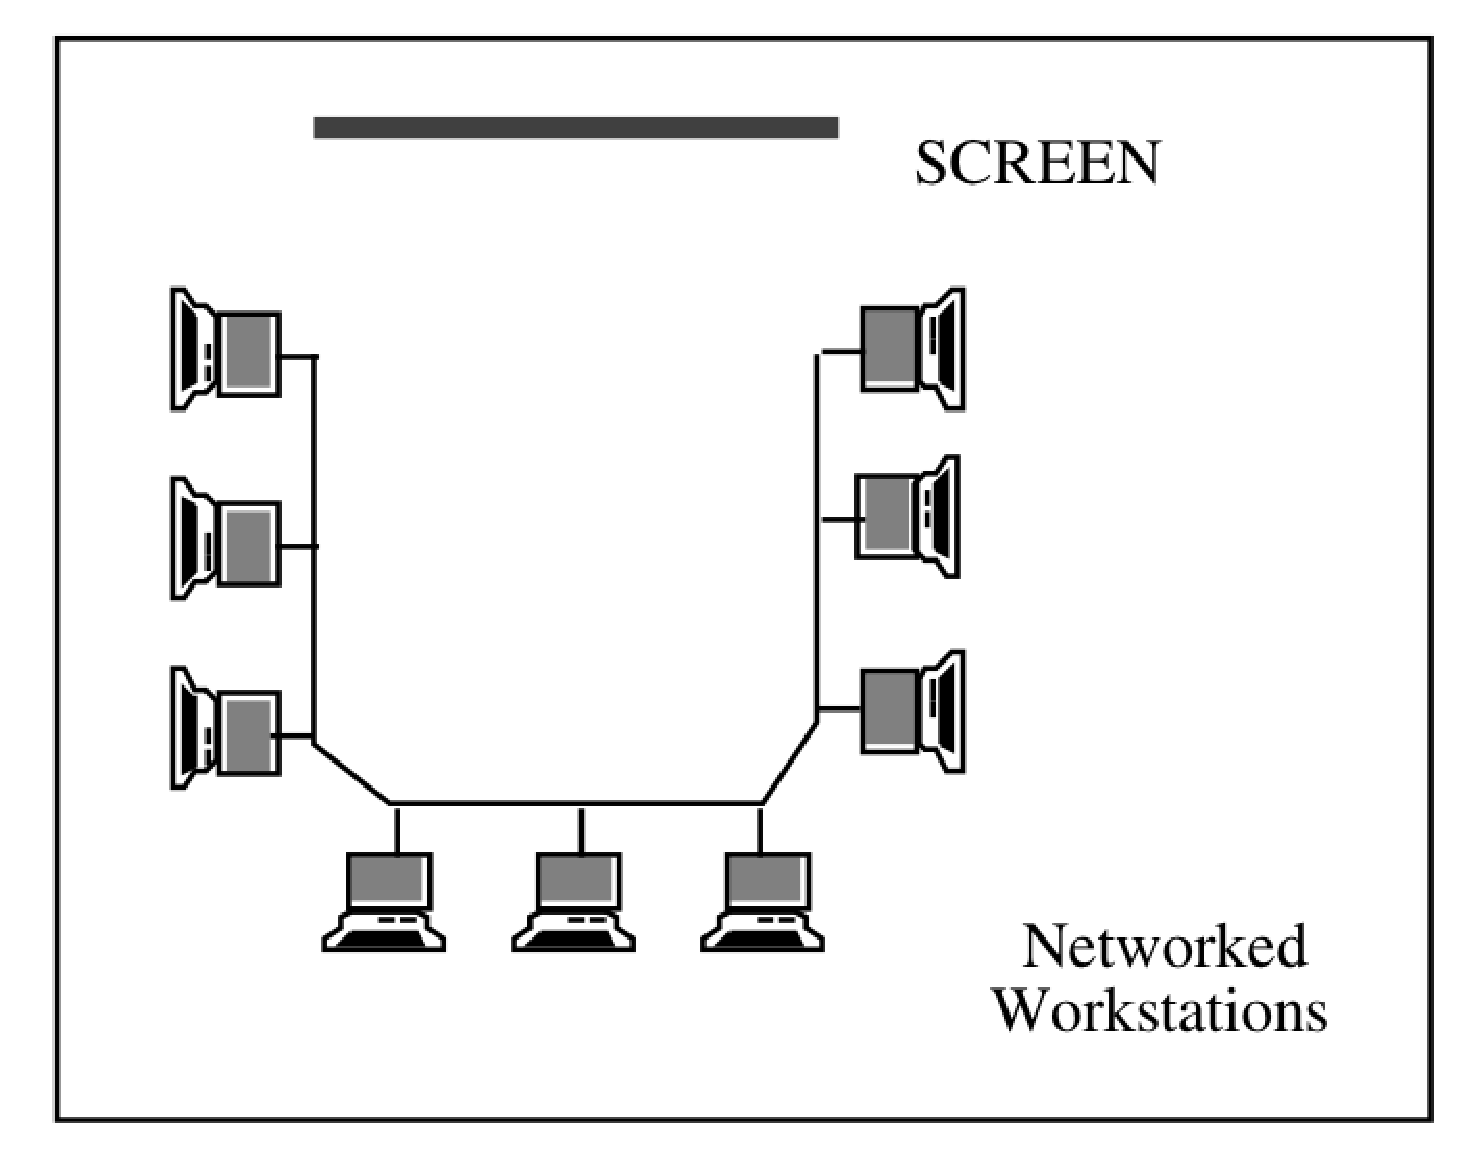
\includegraphics[scale=.5]{meeting_room_sys.eps}
  \label{meeting_room_fig}
\end{figure}

%Describe colab: 

%1) Talk about the objectives

CoLab\cite{Stefik:1987:BCU} is one of the earliest example of a
meeting room system. It aimed to explore the area of using computers
in meeting rooms to carry out tasks that generally required media like
chalk boards. Although the use of chalkboards and similar media
helped the group focus they had their drawbacks for example; the
contents of the chalkboard could not be reproduced once erased,
rearranging items on a chalk board is inconvenient. 

%2) Features 
CoLab attempted to provide a way around these drawbacks by having
shared memory where participants of a conference interacted with one
another. This lead to investigating a multi-user interface where users
could interact with one another using a computer. This further lead to
investigating the field of What You See Is What I See(WYSIWIS). The
outcome of this investigation was that implementing strict WYSIWIS
interfaces was limiting. Instead the designers opted for a more relaxed
interpretation of WYSIWIS where every user apart from interacting with
one another in a shared display also had private windows. 

Since CoLab allowed a number of collaborators to interact with one
another it had consider conflicts between individual users trying to
modify the same object at the same time. As a result the team
experimented with a number of mechanisms to maintain
concurrency, these mechanisms are listed in \cite{Stefik:1987:BCU}.

%3) Describe the components -- Not required, these are tools and as
%such do not add to the discussion.
%  3.1) CogNoter
%  3.2) ArgNoter

\subsection{Co-authoring Systems}

A number of projects can be accomplished only by the effort of a
number of authors. Co-authoring systems are a class of systems that
help support such activity. A wiki can be considered an example of
such a system. A wiki Any user can read an article and when required, they
can modify the content of the article. A wiki also provides space for
authors to discuss the article by providing a separate space for
comments. A wiki provides version and configuration control by means
of saving the updates made to a given document.

\section{Coglaborate}

% Use this section to describe the goals of coglaborate and show which
% class of systems does coglaborate fall under.

Coglaborate aims to enable collaboration between cognitive scientists
who build computational models of their work. Currently these users
are restricted to sharing knowledge via annual conferences,
workshops, summer school and model code distributed via web sites. The
aim of this project is to develop a collaborative modeling environment
for  in which they can develop and share models. 

% Goals of coglaborate
% Provide collaboration for people working in the area of cognitive
% modeling

% Features of coglaborate

Coglaborate currently provides the following features, these are
described in detail in Chapter \ref{chap-five}.
% Users a provided with a lisp listener where they can evaluate their
% code directly

% The users use a customized version of ACT-R that insulates models
% from colliding with each other when running

% The users can evaluate the model immediately and see the result
% immediately

% Once evaluated any user on the system can search and obtain the code
%   for it from the frame representation of the model.

\begin{itemize}
\item A live lisp listener in a web browser where code can be evaluated.
\item A structured representation for models using frames.
\item An intuitive method for sharing and examining models at any
  level of detail.
\end{itemize}

Coglaborate provides support for collaboration by compiling the user's
models into a frame based representation. These representations are
stored in a common area of the memory of the system. Any user who is
familiar with the name of the model, can search for the model and
convert the model to code. This code can then be edited and
recompiled, as a result of this process the original representation is
modified to reflect the change.

Coglaborate can be classified as a co-authoring system. The rationale
behind choosing this classification is that different users can build
the same models incrementally by adding productions or editing
existing models. The following chapter will examine in detail the
design and implementation of the system.
% How does it do it
% Converts all models into frames when evaluated and as a result
% anyone else can search for the frame and manipulate it, re-eval it
% and share it out.

% as a result in its current form Coglaborate is a asynchronous
% co-authoring system because you can have multiple authors working on
% a model.